\documentclass[10 pt, twocolumn]{article}
\documentclass[10 pt, twocolumn]{article}

\usepackage[utf8]{inputenc}
\usepackage[T1]{fontenc}
\usepackage{caption}
\usepackage{graphicx}
\usepackage{xcolor}
\usepackage{interval}
\usepackage{listingsutf8}
\usepackage{hyperref}
\usepackage{siunitx}
\usepackage{algorithm2e}
\usepackage{rotating}
\usepackage{adjustbox}
\usepackage{booktabs}
\usepackage{pgfplots}
\usepackage{tikz}
\usepackage{footmisc}
\usepackage{amsfonts}
\usepackage[backend=biber,style=numeric]{biblatex}
\usepackage[
  left=1.50cm,
  right=1.50cm,
  top=2.00cm,
  bottom=2.00cm
]{geometry}

\pgfplotsset{compat=1.15}

\sisetup{load-configurations=abbreviations, binary-units=true}
\intervalconfig {
    soft open fences ,
    separator symbol =; ,
}

\lstdefinelanguage{JavaScript}{
  keywords={break, case, catch, continue, debugger, default, delete, do, else, finally, for, function, if, in, instanceof, new, return, switch, this, throw, try, typeof, var, void, while, with},
  morecomment=[l]{//},
  morecomment=[s]{/*}{*/},
  morestring=[b]',
  morestring=[b]",
  sensitive=true
}

\lstdefinelanguage{Protobuf}{
  keywords={message, string, uint32, int32},
  morecomment=[l]{//},
  morecomment=[s]{/*}{*/},
  morestring=[b]',
  morestring=[b]",
  sensitive=true
}

\lstset{
    language=C,
    keywordstyle={\bfseries},
    basicstyle=\footnotesize,
    literate={->}{$\rightarrow{}$}{1} {<-}{$\leftarrow{}$}{1},
    stringstyle=\color{purple},
    keepspaces=true,
    captionpos=b,
    inputencoding=utf8,
    escapeinside={\%*}{*)}
}

\renewcommand\AlCapSty{\text}
\SetAlCapNameFnt{\footnotesize}
\SetAlCapFnt{\footnotesize}
\SetAlgoCaptionSeparator{.}
\DeclareCaptionLabelFormat{nospace}{#1 #2}
\captionsetup[table]{labelformat=nospace,labelfont=rm,name=Table,labelsep=period}

\newcommand{\pcode}[1]{
    \lstinline[basicstyle=\itshape,keywordstyle={}]{#1}
}

\newcommand*{\lstnumberautorefname}{line}

\newcommand{\icode}[1]{\lstinline{#1}}

\newcommand{\name}[1] {\emph{#1}}

\newcolumntype{R}[2]{%
    >{\adjustbox{angle=#1,lap=\width-(#2/2)}\bgroup}%
    l%
    <{\egroup}%
}
\newcommand*\rot{\multicolumn{1}{R{90}{1em}}}

\newcommand{\fig}[3]{
  \begin{figure}[h]
    \begin{center}
        \includegraphics[width=8cm,keepaspectratio]{#1}
        \caption{#3}
        \label{fig:#2}
    \end{center}
  \end{figure}
}

\usepackage[most]{tcolorbox}
\newcounter{example}
\usepackage{xparse}
\usepackage{lipsum}

\def\exampletext{Example} % If English
\NewDocumentEnvironment{example}{ O{} }
{
\colorlet{colexam}{red!55!black} % Global example color
\newtcolorbox[use counter=example]{examplebox}{%
    % Example Frame Start
    empty,% Empty previously set parameters
    title={#1},% use \thetcbcounter to access the example counter text
    % Attaching a box requires an overlay
    attach boxed title to top left,
       % Ensures proper line breaking in longer titles
       minipage boxed title,
    % (boxed title style requires an overlay)
    boxed title style={empty,size=minimal,toprule=0pt,top=4pt,left=3mm,overlay={}},
    coltitle=colexam,fonttitle=\bfseries,
    before=\par\medskip\noindent,parbox=false,boxsep=0pt,left=3mm,right=0mm,top=2pt,breakable,pad at break=0mm,
       before upper=\csname @totalleftmargin\endcsname0pt, % Use instead of parbox=true. This ensures parskip is inherited by box.
    % Handles box when it exists on one page only
    overlay unbroken={\draw[colexam,line width=.5pt] ([xshift=-0pt]title.north west) -- ([xshift=-0pt]frame.south west); },
    % Handles multipage box: first page
    overlay first={\draw[colexam,line width=.5pt] ([xshift=-0pt]title.north west) -- ([xshift=-0pt]frame.south west); },
    % Handles multipage box: middle page
    overlay middle={\draw[colexam,line width=.5pt] ([xshift=-0pt]frame.north west) -- ([xshift=-0pt]frame.south west); },
    % Handles multipage box: last page
    overlay last={\draw[colexam,line width=.5pt] ([xshift=-0pt]frame.north west) -- ([xshift=-0pt]frame.south west); },%
    }
\begin{examplebox}}
{\end{examplebox}\endlist}

\newcommand*\circled[1]{\tikz[baseline=(char.base)]{
            \node[shape=circle,draw,inner sep=1pt] (char) {#1};}}

\usepackage{tikz}

\newcommand{\smiley}{\tikz[baseline=-0.75ex,black]{
    \draw circle (2mm);
\node[fill,circle,inner sep=0.5pt] (left eye) at (135:0.8mm) {};
\node[fill,circle,inner sep=0.5pt] (right eye) at (45:0.8mm) {};
\draw (-145:0.9mm) arc (-120:-60:1.5mm);
    }
}

\newcommand{\frownie}{\tikz[baseline=-0.75ex,black]{
    \draw circle (2mm);
\node[fill,circle,inner sep=0.5pt] (left eye) at (135:0.8mm) {};
\node[fill,circle,inner sep=0.5pt] (right eye) at (45:0.8mm) {};
\draw (-145:0.9mm) arc (120:60:1.5mm);
    }
}

\newcommand{\neutranie}{\tikz[baseline=-0.75ex,black]{
    \draw circle (2mm);
\node[fill,circle,inner sep=0.5pt] (left eye) at (135:0.8mm) {};
\node[fill,circle,inner sep=0.5pt] (right eye) at (45:0.8mm) {};
\draw (-135:0.9mm) -- (-45:0.9mm);
    }
}


\addbibresource{root.bib}

\title{Integrating microservices}

\author{Jan Mach{\'a}\v{c}ek%$^{1}$% <-this % stops a space
\thanks{Supported by BAMTECH Media}% <-this % stops a space
\thanks{$^{1}$J. Machacek is the Senior Principal Engineer at BAMTECH Media, Houldsworth Mill, Houldsworth Street, Reddish, SK5 6DA, UK {\tt\small jan.machacek at bamtechmedia.com}}%
}

\begin{document}

\twocolumn[
  \begin{@twocolumnfalse}
    \maketitle
    \begin{abstract}
      When a system needs to spread across asynchronous and unreliable communications boundary, its components on either side of this boundary have to use precise API. The protocol

      Kafka is cool. Now, how to use it, run it, and what are the pitfalls.
    \end{abstract}
  \end{@twocolumnfalse}
]

\section{Stateful distributed systems}
Systems whose components run on multiple nodes are difficult to design without obvious errors, difficult to build, difficult to run, and difficult to maintain; the reasons that justify this complexity are resilience and performance. Resilience refers to the system's ability to continue to operate even if some of its components are failing; informally, performance refers to the system's ability to handle large incoming workload quickly. The exact definitions for ``large'' and ``quickly'' <- TODO.

\autoref{tbl:ll-latency}\cite{fommil-netlib} shows typical latencies in a computer system translated to human timescales; it demonstrates that ``the further the CPU has to go, the longer it takes''.

\begin{table}[h]
    \begin{tabular}{p{3cm}lp{3.5cm}}
        \toprule
        Computer & Human & Analogy \\
        \midrule
L1 cache reference & \SI{0.5}{\second} & One heart beat \\
Branch mispredict  & \SI{5}{\second} & Yawn \\
L2 cache reference & \SI{7}{\second} & Long yawn \\
Mutex lock/unlock  & \SI{25}{\second} & Making a cup of tea \\
        \midrule
Main memory reference & \SI{100}{\second} &  Brushing one's teeth \\
Compress \SI{1}{\kibi\byte} with Zippy & \SI{50}{\minute} & Build Scala \\
Send \SI{2}{\kibi\byte} over \SI{1}{\giga\bit\per\second} network & \SI{5.5}{\hour} & London to Edinburgh \\
        \midrule
SSD random read & \SI{1.7}{\day} & Weekend \\
Read \SI{1}{\mebi\byte} sequentially from memory & \SI{2.9}{\day} & Long weekend \\
Round trip within same datacentre & \SI{5.8}{\day} & Short holiday \\
Read \SI{1}{\mebi\byte} sequentially from SSD & \SI{11.6}{\day} & Holiday \\
        \midrule
Disk seek & \SI{16.5}{w} & Term of university \\
Read \SI{1}{\mebi\byte} sequentially from disk & \SI{7.8}{m} & Fully paid maternity in Norway \\
Send packet CA $\rightarrow$ Netherlands $\rightarrow$ CA & \SI{4.8}{y} & Government's term \\
        \bottomrule
    \end{tabular}
    \caption{Low-level latency}
    \label{tbl:ll-latency}
\end{table}

XXX

\begin{table}[h]
    \begin{tabular}{lrrrrrr}
        \toprule
        Program           & \multicolumn{6}{c}{Implementation \& Runtime} \\
        \cmidrule(r){2-7} & Scala  & Go  & C++ & Haskell & Python & JavaScript \\
        \midrule
        Simple            1.00   & 3.84    & 1.86  & 3.97   & 0 & 0 \\
        Some exceptions   5.16   & 8.02    & 2.26  & 3.93   & 0 & 0 \\
        All exceptions    42.51  & 66.00   & 4.12  & 3.93   & 0 & 0 \\
        Enterprise        3.00   & 25.12   & 2.24  & 3.92   & 0 & 0 \\
        Bad async         868.50 & 959.99  & 44.30 & 615.51 & 0 & 0 \\
        \bottomrule
    \end{tabular}
    \caption{Runtime}
    \label{tbl:code-style-impact}
\end{table}

\begin{figure}[h]
  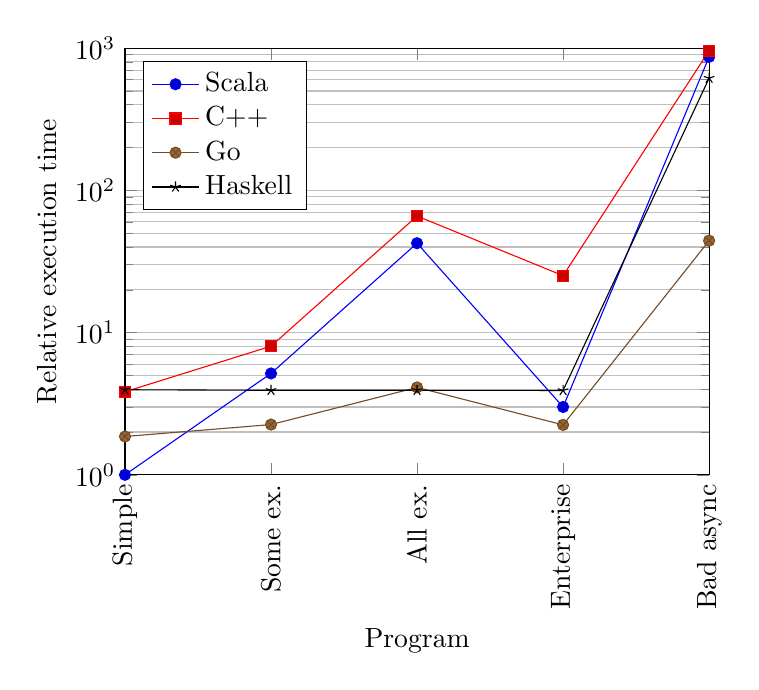
\begin{tikzpicture}
    \begin{axis}[
      height=7cm, 
      width=9cm, 
      yminorgrids=true,
      xtick=data,
      ymode=log,
      xlabel={Program}, 
      ylabel={Relative execution time},
      ymin=1,ymax=1000,
      xmin=0,xmax=4,
      legend pos=north west,
      legend cell align={left},
      xticklabel style={rotate=90},
      xticklabels={Simple, Some ex., All ex., Enterprise, Bad async}
      ]

      \addplot+ coordinates {
        (0, 1)
        (1, 5.162790698)
        (2, 42.51162791)
        (3, 3)
        (4, 868.5)
      };
      \addlegendentry{Scala}

      \addplot+ coordinates {
        (0, 3.837209302)
        (1, 8.023255814)
        (2, 66)
        (3, 25.12790698)
        (4, 959.9883721)
      };
      \addlegendentry{C++}

      \addplot+ coordinates {
        (0, 1.860465116)
        (1, 2.255813953)
        (2, 4.11627907)
        (3, 2.244186047)
        (4, 44.30232558)
      };
      \addlegendentry{Go}

      \addplot+ coordinates {
        (0, 3.965116279)
        (1, 3.930232558)
        (2, 3.930232558)
        (3, 3.918604651)
        (4, 615.5116279)
      };
      \addlegendentry{Haskell}
    \end{axis}
  \end{tikzpicture}
  \caption{Simple computation}
  \label{plot:simple-computation}
\end{figure}

\twocolumn[
\begin{@twocolumnfalse}
\begin{figure}[h]
  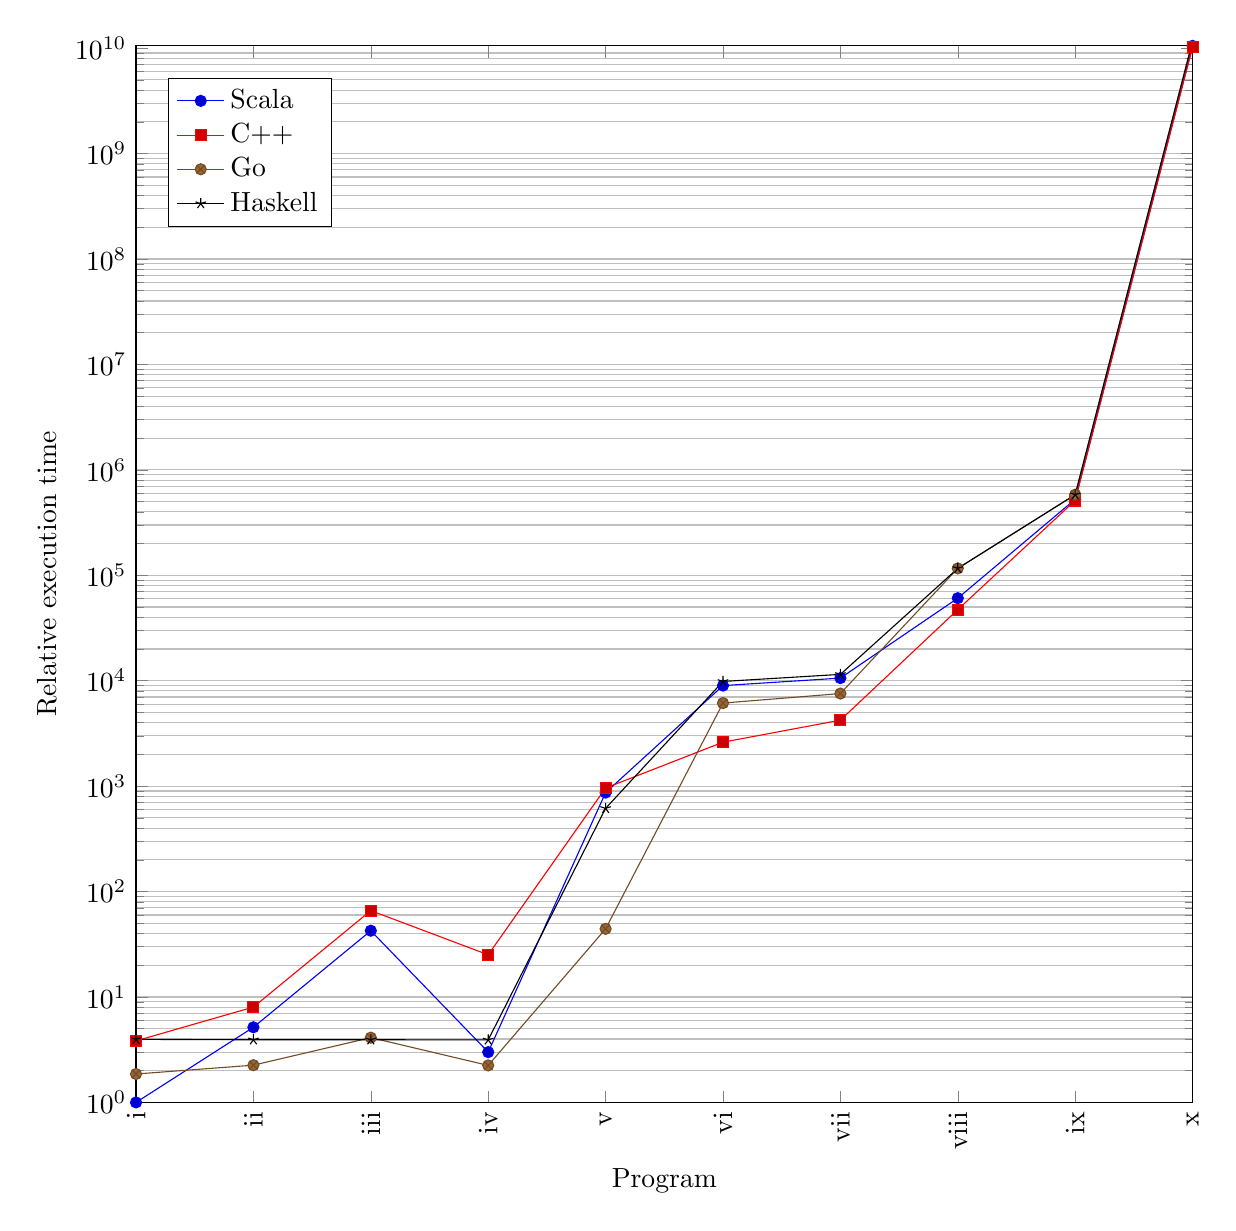
\begin{tikzpicture}
    \begin{axis}[
      height=15cm, 
      width=15cm, 
      yminorgrids=true,
      xtick=data,
      ymode=log,
      xlabel={Program}, 
      ylabel={Relative execution time},
      ymin=1,ymax=10516002326,
      xmin=0,xmax=9,
      legend pos=north west,
      legend cell align={left},
      xticklabel style={rotate=90},
      xticklabels={ i, ii, iii, iv, v, vi, vii, viii, ix, x}
      ]

      \addplot+ coordinates {
        (0, 1)
        (1, 5.162790698)
        (2, 42.51162791)
        (3, 3)
        (4, 868.5)
        (5, 8988.348837)
        (6, 10586.84884)
        (7, 60683.83721)
        (8, 525800.1163)
        (9, 10516002326)
      };
      \addlegendentry{Scala}

      \addplot+ coordinates {
        (0, 3.837209302)
        (1, 8.023255814)
        (2, 66)
        (3, 25.12790698)
        (4, 959.9883721)
        (5, 2610.965116)
        (6, 4225.232558)
        (7, 47250.87209)
        (8, 512367.1512)
        (9, 10247343023)
      };
      \addlegendentry{C++}

      \addplot+ coordinates {
        (0, 1.860465116)
        (1, 2.255813953)
        (2, 4.11627907)
        (3, 2.244186047)
        (4, 44.30232558)
        (5, 6135.988372)
        (6, 7553.034884)
        (7, 116279.0581)
        (8, 581395.3372)
        (9, 11627906744)
      };
      \addlegendentry{Go}

      \addplot+ coordinates {
        (0, 3.965116279)
        (1, 3.930232558)
        (2, 3.930232558)
        (3, 3.918604651)
        (4, 615.5116279)
        (5, 9842.953488)
        (6, 11480.0814)
        (7, 116279.0581)
        (8, 581395.3372)
        (9, 11627906744)
      };
      \addlegendentry{Haskell}
    \end{axis}
  \end{tikzpicture}
  Where 
  \begin{enumerate}[i]
    \item Simple
    \item Some ex.
    \item All ex.
    \item Enterprise
    \item Bad async
    \item \SI{1}{\mebi\byte} from \pcode{/dev/zero}
    \item \SI{1}{\mebi\byte} from regular file
    \item REST API call with \SI{100}{\micro\second} latency
    \item REST API call with \SI{10}{\milli\second} latency
    \item REST API call with \numprint{0.00001} error rate + \SI{10}{\milli\second} latency
  \end{enumerate}
  \caption{Simple computation}
  \label{plot:simple-computation}
\end{figure}
\end{@twocolumnfalse}
]

\section{State in distributed system}
Imagine two systems that need to share information; a good starting point may be an endpoint where one system can request the state of the other system. If the first system needs to keep ``in sync'' with the second system, it needs to periodically query the endpoint to obtain the state from the second system. This keeps the two systems independent and decoupled, but it means that the systems might miss important state changes that happen between the two polls, and it makes both systems do needless work by querying the endpoints, even if the state remains the same.

This inefficiency, the complexity of building reliable and easy-to-use endpoints, the reasoning that both systems are views on the same underlying data, the possible time-pressures to deliver working integration, leads to the \emph{database as integration layer} anti-pattern\cite{eip}. Never mind the \emph{anti} in anti-pattern: what would happen if the systems actually decided to use a shared database? As the database spreads over multiple networked nodes, which introduces unreliability and delay, and means that the database administrators now need to choose the two of the C$\cdot$A$\cdot$P (C stands for consistency, A for availability, and P for partition-tolerance)--as long as one of the choices is P. This leaves the DBAs with a decision between A and C. A database that keeps its state on multiple nodes may keep them ``in sync'' by sending the nodes messages that describe the state transitions to be applied to the state. The state that the database (in the sense of all its nodes) keeps is then simply a reliable playback of all the messages. The state is a snapshot of the stream of messages at a given point in time. However, the decision between C and A still remains. If the choice is C, then all nodes have to agree that they have indeed received and applied all messages up to some point in time; in case the messages aren't received, or if there is no agreement, the database must become unavailable. If the choice is A, then there is the risk that a node that is being queried has not yet received all update messages; querying another node may yield different result; repeating the same query on the original node later may yield different result.

Using a database as an integration layer does not make the difficult choices of a distributed system go away, yet it keeps all the disadvantages of the anti-pattern. It forces shared data model, which may couple two (multiple!) systems together in the same release cycle; it is also a recipe for slowly-growing monolith, where one of the systems gains more and more functionality (the one with the largest number of developers); the other systems become lighter--after all, they are just views on the same shared state. The shared data model also means that two (multiple!) systems have to agree on usable data models for each.

\section{Message-driven systems}
If the systems that are to be integrated are event-driven--each system publishes messages as it proceeds with its operation, and if each system accepts messages at any time without previously initiating a request--then the integration can take advantage of this transfer of information. Relying entirely on [persistent] messaging can be burdensome; it is reasonable to rely on snapshots to remove the need to replay the messages from the beginning of time at start-up. 

It might seem reasonable to rely on an endpoint that can deliver the entire snapshot in one response at start-up. Ignoring the potential problems with the size of the response, this will make the two systems to be integrated more coupled together. Specifically, it will remove the decoupling in time that the persistent messaging mechanism brings. 

Consider two systems that need to share parts of their state. If both systems are event-driven, the task is simpler: all that needs to be done is to deliver the messages from the first system to the second system. Even though it is possible for the second system to accept the ``internal'' messages from the first system, it is safer to add a component that implements translation between the two systems. (This translation component can be \pcode{identity}, but it should be there.) \autoref{fig:2s-es} illustrates the event-driven scenario.

\fig{2s-es.png}{2s-es}{Integrating two systems}

Both systems \circled{A} and \circled{B} have their private journal and snapshot stores. The sharing of state begins by initial query that pulls in the appropriate snapshot of state from system \circled{A} into \circled{B} in \circled{1}; then the system \circled{B} follows the state changes in \circled{A} by acting on the [translated] messages it receives from \circled{A}. The system \circled{A} is not aware of any connection; it is not even aware of the translation component; all that the system \circled{A} is concerned about is delivery of messages to its messaging boundary. The flow is illustrated in \circled{2}, \circled{3}, and \circled{4}.

\autoref{fig:2s-es} does not explain how the messages cross the boundary between the systems; it is clear that there needs to be some kind of connector that sits either on the \circled{A} or the \circled{B} side. It is better for the connector to be on the \circled{B} side. \circled{B} wants to receive messages from \circled{A}, so it should be responsible for making the arrangements: it should verify that it is indeed connecting to the \emph{right} \circled{A} (checking certificates, for example); even more importantly, the connector needs to \emph{consume} messages from \circled{A}, and then \emph{publish} the same messages to \circled{B}. Publishing is potentially much more complex procedure (what is the acceptable confirmation / acknowledgement, what are the maximum batch sizes, time-outs, etc.), and should be in full control of \circled{B}\cite{mirrormaker}.  

% If the two systems are not event-driven, but rather simpler CRUD-based services, it may be possible to pull the state update messages from the data stores that the systems use; either using the datastore's native functionality or by implementing a custom service. Ideally, the only change to the integration flow will be the source and destination of the messages: the source becomes the state database in \circled{A}; the destination becomes \circled{B}'s APIs (see \autoref{fig:2s-crud}). 

% \fig{2s-crud.png}{2s-crud}{Integrating CRUD systems}

All other approaches are recpies for problems (now or in the very near future). By far the worst-case scenario is database-to-database integration; particularly where \circled{A} writes directly to the database of \circled{B}. This is the most brittle and most dangerous approach; only slightly less dangerous and brittle solution is for \circled{B} to pull data from \circled{A}'s database. If the system \circled{B} is not event-driven, the only approach is to poll data from \circled{A}\footnote{To avoid the inefficiency of frequent polls with no changes, or too infrequent polls missing changes, add a component that can act as fancy circuit-breaker}. 

If the two systems are connected ``from the beginning of time'' (that is \circled{B} receives all messages from \circled{A} from the first message), or if the two systems only need to synchronise a fixed number of messages, there will be no need to worry about the initial snapshot poll from \circled{A}. In other cases, \circled{B} requests the initial state from \circled{A} and then subscribes to the updates. Unfortunately, \circled{A} keeps updating its state, even as it serves the response to the initial poll to \circled{B}. A simple algorithm that \circled{A} can follow--\pcode{state <- poll(B); subscribe(B);}--runs the risk of missing messages that happened just after the initial poll. A systematic way of solving this is to include an offset in the initial poll response specifying the position at which the snapshot was taken. \circled{B} is responsible for subscribing to updates from \circled{A} from that offset. This way, there is no risk in missing updates from \circled{A}. An alternative is to measure the risk of missing an update vs. doing too much work and subscribing from the end of the topic less some arbitrary offset.

A typical event-driven system with persistent messaging implemented in Kafka typically uses multiple topics, each with multiple partitions. The offset is associated with each topic partition; the response to the initial poll request needs to to include a map of \pcode{(topic, partition) -> offset}. \autoref{fig:2s-es-msgs} illustrates the message contents and flow.

\fig{2s-es-msgs.png}{2s-es-msgs}{Messages}

The first message is the response to the request for initial state. It contains the state (in the \pcode{body} field) and the topic partition offsets used to construct the state. After processing the initial state \circled{B} subscribes to the topics indicated by \circled{A} to receive updates. This gurarantees that no messages will be lost, though it does not guarantee a \emph{total ordering} of the update messages on the topic; \circled{B} has to be able to deal with out-of-order delivery of the update messages\footnote{Distributed messaging systems such as Kafka\cite{kafka} or AWS Kinesis\cite{kinesis} only have total order in a specific partition of a topic.}. \autoref{code:2s-es-msg-flow} shows a typical code in \circled{B}.


\begin{lstlisting}[caption={Message flow}, label={code:2s-es-msg-flow}, language=Pseudo, escapechar=|]
if not initialised then 
    (tps, state) <- poll(A)
    insert(state)
    subscribe(mode = SemiAutomatic, tpos = tpos, 
              onMessage = /\m -> update(m))
else
    subscribe(mode = FullyAutomatic,
              onMessage = /\m -> update(m))
end if
\end{lstlisting}

The \pcode{not initialised} indicates that \circled{B} has never been synchronised with A; the \pcode{mode = SemiAutomatic} instructs the messaging infrastructure to handle offset management, but allow initial offset specification; the \pcode{mode = FullyAutomatic} indicates that the messaging infrastructure should start the subscription from the last consumed offset.

\section{Implementation}
This paper will offer two implementation approaches: one that relies on Apache Kafka and one that uses the AWS tooling. Other implementations will find many common principles between the two.

\subsection{Kafka-based}
If the system cannot take advantage of any built-in functionality to the underlying infrastructure, it will be necessary to build the connectors and transformers ourselves. 

System 1 <=> MySQL
          -> Kafka => Mirror Maker -> Kafka Connector -> Kafka -> Kafka Connector -> MySQL <=> System 2

\subsection{AWS-based}

System 1 <=> Dynamo 
          -> Kinesis => Kinesis Replicator -> Lambda -> Kinesis -> Lambda -> MySQL <=> System 2

\section{Scalability and resilience}
TODO.

\section{Practical applicaiton}
X requested a feature in the Y system to implement a REST API endpoint that can be queried for the current state of a particular media assignment; but this request should also create a subscription for any changes to be delivered to the X system over a Kafka topic. The motivation for the feature was X’s need to know Y’s state, but to avoid doing periodic polling. (Polling, the team X reasoned, is just not cool, and might still miss an important change that happens between the two polls.)
\begin{itemize}
  \item Y should not implement state that is only useful for X. The state Y would hold is not needed for its operation, it only serves one particular client;
  \item Maintaining subscriptions requires more state to be maintained inside Y; this state needs to be recoverable in case of failures, adding significant complexity to Y;
  \item  Even with the subscription in place, the system (comprising Y and X) remains eventually consistent; adding arbitrary delays to the subscription does not solve this. (e.g. only start sending updates 40 seconds later to be sure that there was enough time for the state to become consistent does not solve the problem of eventual consistency; it simply allows us to pretend that the system is consistent!)
  \item There is no clear understanding (maybe there cannot be clear understanding) of when a subscription ends, or what identifies a client
\end{itemize}
Instead, I guided the teams to understand a better approach (bite the bullet and have X subscribe to the existing updates topic and maintain its own model, which duplicates information in principle, but allows most suitable representation of the information to exist in each system; it also maintains clear separation of responsibilities of each system; finally, it does not lock the two systems in the same release cycle).


\printbibliography

\end{document}